\documentclass{article}
\usepackage{amsmath}
\usepackage{mathtext}
\usepackage[T1,T2a]{fontenc}
\usepackage[utf8]{inputenc}
\usepackage[english, bulgarian, russian]{babel}
\usepackage{tikz}
\usepackage{pgfplots}
\usepackage[export]{adjustbox}
\usepackage{siunitx}
\usepackage{booktabs}
\usepackage{pgfplotstable}
\usepackage[left=2cm,right=2cm,
    top=2cm,bottom=2cm,bindingoffset=0cm]{geometry}
    

\title{Лабораторная работа 1.2.5\\Исследование прецессии уравновешенного гироскопа}
\date{9.12.2019}
\author{Панферов Андрей}

\begin{document}
  \pagenumbering{gobble}
  \maketitle
  \newpage
  \pagenumbering{arabic}
  
  

\section{Аннотация}

В работе исследуется вынужденная прецессия гироскопа. Устанавливается зависимость скорости вынужденной прецессии от величины момента сил, действующих на ось гироскопа. Определяется скорость вращения ротора гироскопа и сравнивается со скоростью, рассчитанной по скорости прецессии. 


\section{Теоретические сведения}

Так как уравнения движения твердого тела можно записать в виде. 

\begin{center}

  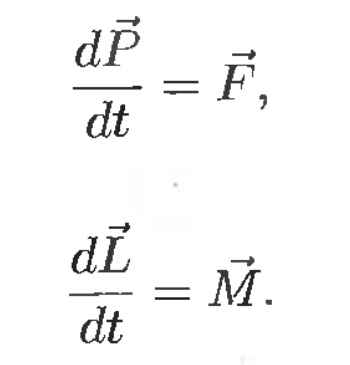
\includegraphics[width=0.1\linewidth]{IMG_1.jpg}\\
 
 \end{center}


Этих двух уравнений достаточно для полного описания состояния его движения. 

Так как если сила не зависит от угловой скорости, а момент -- от скорости поступательного движения, то эти уравнения можно рассматривать независимо друг от друга. 
Момент импульса твердого тела в его главных осях x, y, z равен

\begin{center}

  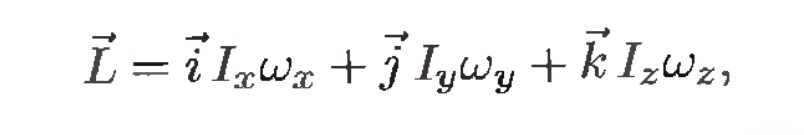
\includegraphics[width=0.4\linewidth]{IMG_2.jpg}\\
 
 \end{center}
Под действием момента внешних сил ось гироскопа медленно вращается вокруг оси у с угловой скоростью \Omega. Для гироскопа  массой $m_г$, у которого ось собственного вращения наклонена на углол \alpha от вертикали, скорость прецессии, происходящей вокруг вертикальной оси под действием силы тяжести, равна. 

\begin{center}
  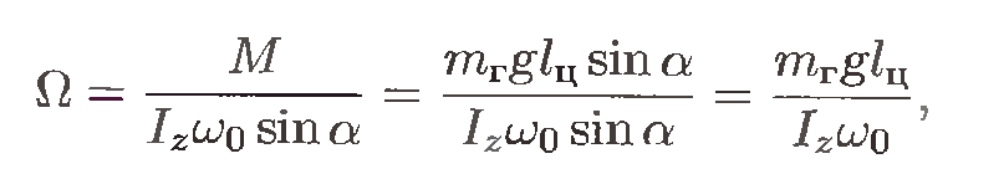
\includegraphics[width=0.4\linewidth]{IMG_3.jpg}\\
 
 \end{center}

\begin{center}

  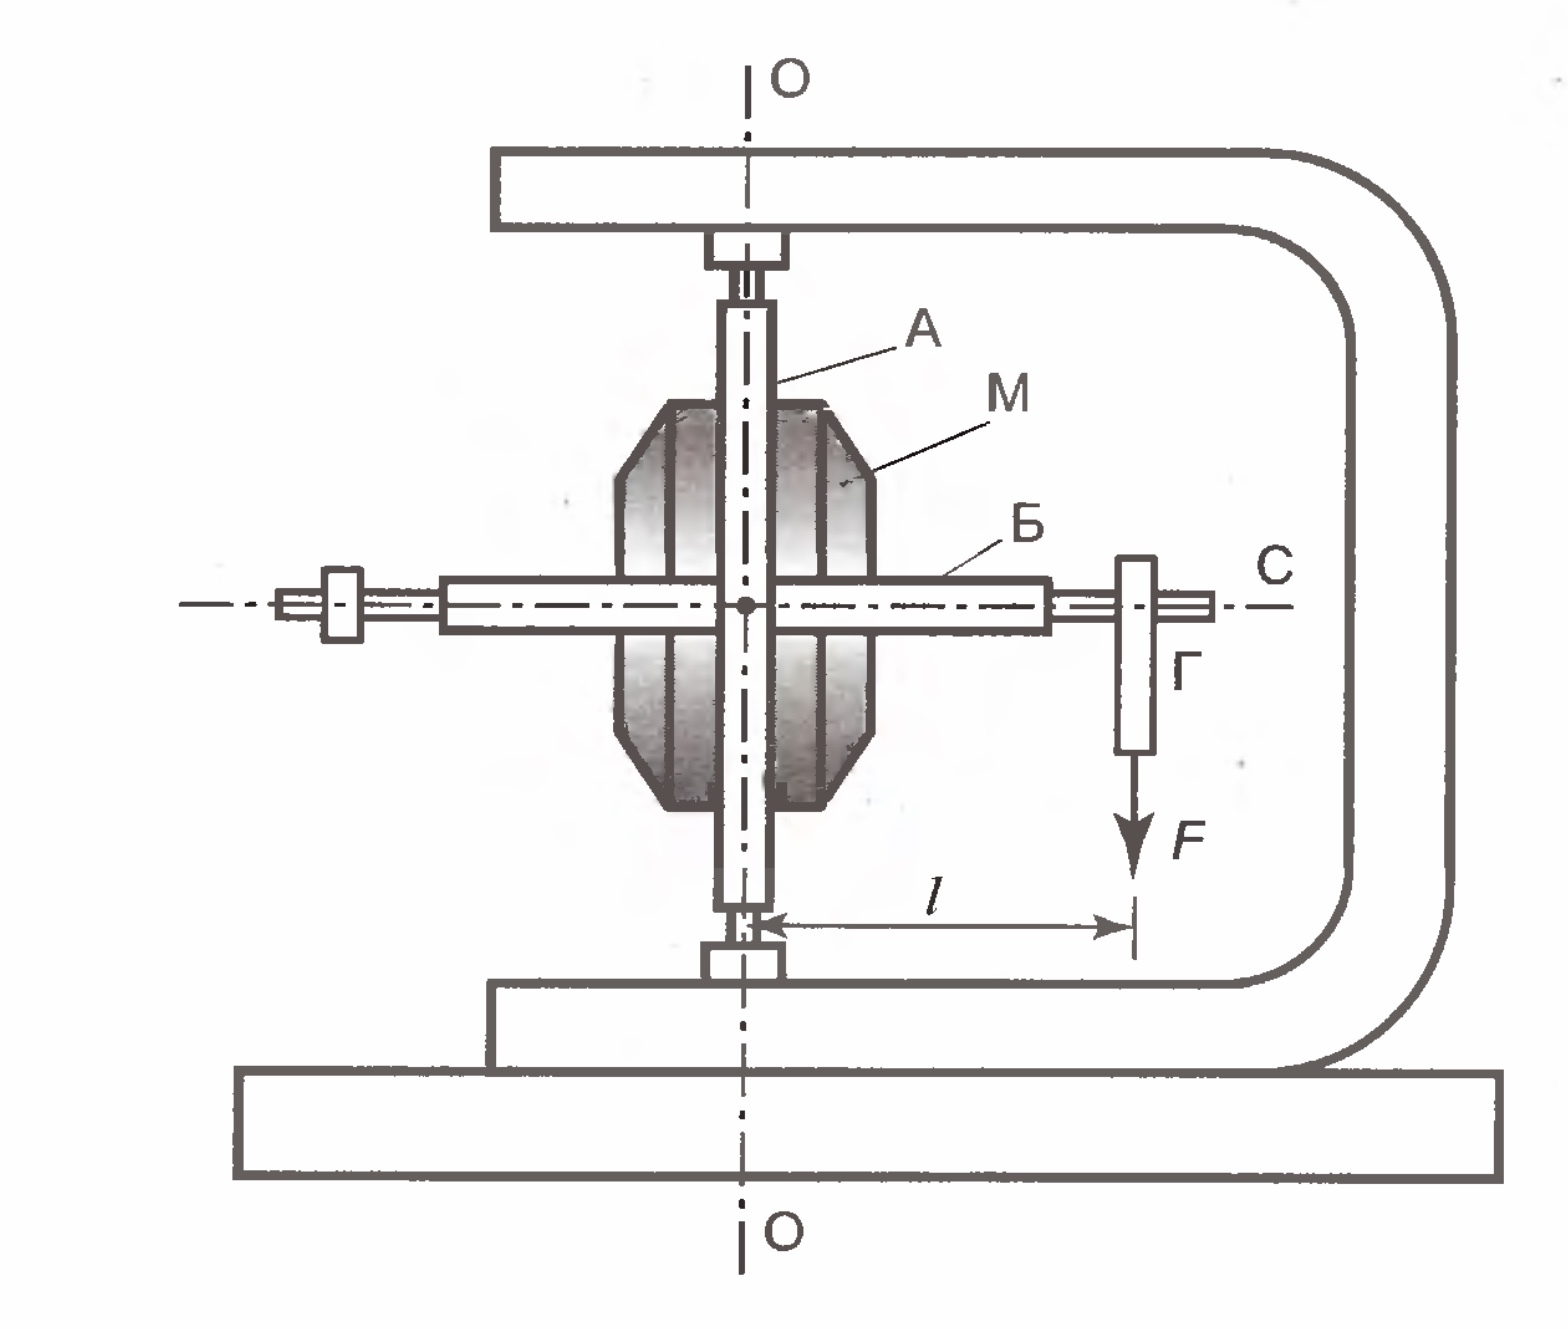
\includegraphics[width=0.5\linewidth]{IMG_4.jpg}\\
 
  Схема экспериментальной установки\\
 
 \end{center}

В данной работе исследуется регулярная прецессия уравновешенного гироскопа. 
Измерение скорости прецессии гироскопа позволяет вычислить угловую скорость вращения его ротора. 

\section{Оборудование и инструментальные погрешности}

В работе используются: гироскоп в кардановом подвесе, секундомер, набор грузов, отдельный ротор гироскопа, цилиндр известной массы, крутильный маятник, штангенциркуль, линейка.\\
\\
1. Точность измерения с помощью штангенциркуля -- 0,1 мм. \\
2. Точность измерения с помощью линейки -- 0,5 мм. \\
3. Точность измерения времени -- 0,1 с. \\
4. Точность измерения угла поворота гироскопа вокруг своей оси -- 3 градуса. \\
5. Точность измерения угла поворота во время опускания рычага -- 1 градус. \\
\section{Результаты измерений и обработка данных}
\subsection{Подготовка к эксперименту}
Установим ось гироскопа в горизонтальное положение, осторожно поворачивая ее за рычаг С.
Включим питание гироскопа и подождем несколько минут, чтобы вращение ротора успело стабилизироваться.
Убедимся в том, что ротор вращается достаточно быстро: при легком постукивании по рычагу С последний не изменяет своего положения в пространстве.

Ротор вращается против часовой стрелки. 

При подвешивании к рычагу С груза Г начинается прецессия гироскопа, а трение в горизонтальной оси приводит к тому, что рычаг начинает медленно опускаться.

\subsection{Измерение момента инерции ротора относительно оси симметрии $I_0$}
Повесим ротор, извлеченный из такого же гироскопа, к концу висящей проволоки так, чтобы ось симметрии гироскопа была вертикальна, и измерим период крутильных колебаний получившегося маятника.

\begin{align*}
  30T_2 $=  97,0 \pm 0,5 \ c && T_2 = 3,23 \pm 0,02 \ c\\
\end{align*}

Заменим ротор гироскопа цилиндром, для которого известны данные:

\begin{align*}
  m &= 1617,8 \pm 0,1 \ г & d = 7,8 \pm 0,1 \ см\\
\end{align*}
Где m, h и d -- масса, высота и диаметр цилиндра соответственно.

И проведем аналогичное измерение для цилиндра:

\begin{align*}
  30T_1 $=  118,7 \pm \ 0,5 \ c && T_1 = 3,96 \pm 0,02 \ c\\
\end{align*}


Так как момент инерции цилиндра относительно оси симметрии равен:

\begin{align*}
  I_1 &= \frac{md^2}{8} & I_1 = (1,23 \pm 0,03) \cdot 10^{-3} кг \cdot м^2 \\
\end{align*}

Тогда исходя из формулы вычислим момент инерции ротора $I_2$

\begin{align*}
  I_2 &= I_1 \frac{T_2^2}{T_1^2} & I_2 = (0,82 \pm 0,05) \cdot 10^{-3} кг \cdot м^2 \\
\end{align*}


\subsection{Измерение угловой скорости регулярной прецессии}
Отклоним рычаг на небольшой угол вверх и с помощью секундомера найдем угловую скорость регулярной прецессии $\Omega$ для разных значений приложенного момента сил, приложенных к рычагу С.\\ 

\begin{center}
\begin{minipage}{0.4\textwidth}
\begin{tabular}{|c|c|c|c|}
\hline
 $№$ & $N, обoротов$ & $NT, c$ & $\Delta \phi, град$ \\
\hline 
 1 & 3 & 105.9 &  10\\
\hline
 2 & 3 & 106.3 & 10\\
\hline 
 3 & 3 & 106.1 &  10\\
\hline
 4 & 3 & 106.1 & 10\\
\hline
 5 & 4 & 141.4 & 10\\
\hline
\end{tabular}
\begin{center}
\caption{Масса груза 343г}
\end{center}
\end{minipage}
\begin{minipage}{0.4\textwidth}
\begin{tabular}{|c|c|c|c|}
\hline
 $№$ & $N, обoротов$ & $NT, c$ & $\Delta \phi, град$ \\
\hline 
 1 & 5 & 222.4 & 10\\
\hline
 2 & 3 & 133.3 & 10\\
\hline 
 3 & 3 & 133.2 & 11\\
\hline
 4 & 3 & 133.2 & 10\\
\hline
 5 & 3 & 133.2 & 10\\
\hline
\end{tabular}
\begin{center}
\caption{масса груза 273г}
\end{center}
\end{minipage}
\\
\begin{align*}
\end{align*}
\begin{minipage}{0.4\textwidth}
\begin{tabular}{|c|c|c|c|}
\hline
 $№$ & $N, обoротов$ & $NT, c$ & $\Delta \phi, град$ \\
\hline 
 1 & 4 & 220.3 &  10\\
\hline
 2 & 3 & 164.0 & 11 \\
\hline 
 3 & 3 & 164.7 &  10\\
\hline
 4 & 3 & 164.4 & 10\\
\hline
 5 & 2 & 164.2 & 9\\
\hline
\end{tabular}
\begin{center}
\caption{масса груза 220г}
\end{center}
\end{minipage}
\begin{minipage}{0.4\textwidth}
\begin{tabular}{|c|c|c|c|}
\hline
 $№$ & $N, обoротов$ & $NT, c$ & $\Delta \phi, град$ \\
\hline 
 1 & 3 & 297.5 &  9\\
\hline
 2 & 3 & 206.3 & 10\\
\hline 
 3 & 3 & 206.0 &  9\\
\hline
 4 & 3 & 206.9 & 9\\
\hline
 5 & 3 & 206.6 & 10\\
\hline
\end{tabular}
\begin{center}
\caption{масса груза 176г}
\end{center}
\end{minipage}
\\
\begin{align*}
\end{align*}
\begin{minipage}{0.4\textwidth}
\begin{tabular}{|c|c|c|c|}
\hline
 $№$ & $N, обoротов$ & $NT, c$ & $\Delta \phi, град$ \\
\hline 
 1 & 3 & 256.4 & 10\\
\hline
 2 & 2 & 171.7 & 10 \\
\hline 
 3 & 2 & 171.2 & 10\\
\hline
 4 & 2 & 171.1 & 11\\
\hline
 5 & 2 & 171.5 & 10\\
\hline
\end{tabular}
\begin{center}
\caption{масса груза 142г}
\end{center}
\end{minipage}

\begin{center}
\caption{Усредним значения, пересчитаем данные.}
\end{center}
\\


\begin{center}
\begin{tabular}{|c|c|c|c|c|c|}
\hline
 $m, г$ &$M, мН \cdot м$ & $Т, с$ & $\Omega, \frac{рад}{с}\cdot 10^{-3} $ & $\Delta \phi, град$ & $\Omega_{тр}, \frac{рад}{с} \cdot 10^{-3}$ \\
\hline 
 343 & 403 & $35.4\pm0.3$ & 177.7 & 10 & 4.93 \\
\hline
 267 & 314 & $44.4\pm0.3$ & 141.4 & 10 & 3.93 \\
\hline 
 215 & 253 & $54.8\pm0.3$ & 114.6 & 10 & 3.18 \\
\hline
 141 & 166 & $68.9\pm0.4$ & 74,1 & 10 & 2.53 \\
\hline
 116 & 136 & $85.7\pm0.4$ & 58,0 & 10 & 2.04 \\
\hline
\end{tabular}
\end{center}

\\
\begin{align*}
\end{align*}
\\

\begin{center}
\begin{tikzpicture}[scale = 1.33]
\begin{axis}[
    axis lines = left,
    legend style={at={(0.7,0.9)}},
    xlabel = {$M, мН \cdot м$},
    ylabel = {$\Omega, \frac{рад}{с}\cdot 10^{-3} $
},
    xmin=0, xmax=430,
    ymin=0, ymax=199,
	ymajorgrids = true,
	xmajorgrids = true
]
\addplot[
	mark = square, 
	mark options = {
		scale = 1.5, 
		fill = red, 
		draw = chucknorris
	},
	ymajorgrids = true,
	xmajorgrids = true,
	color = blue 
]  coordinates {
	(403, 177.7) (314, 141.4) (253, 114.6) (166, 74.1) (136, 58.0)};
\addplot
coordinates{(-205,-93)(660,295)}
\legend{ 
	$Зависимость \  \Omega \ от \ М$
};

\end{axis}
\end{tikzpicture}
\end{center}

\begin{center}
\begin{tikzpicture}[scale = 1.33]
\begin{axis}[
    axis lines = left,
    legend style={at={(0.8,1)}},
    xlabel = {$\Omega, \frac{рад}{с}\cdot 10^{-3} $},
    ylabel = {$\Omega_{тр}, \frac{рад}{с}\cdot 10^{-3} $
},
    xmin=0, xmax=200,
    ymin=0, ymax=6,
	ymajorgrids = true,
	xmajorgrids = true
]
\addplot+ [
  error bars/.cd,
      y dir = both, y explicit,
	mark = square, 
	mark options = {
		scale = 1, 
		fill = red, 
	},
	ymajorgrids = true,
	xmajorgrids = true,
	color = blue 
]  coordinates {
	(177.7, 4.93) +- (0, 1)
  (141.4, 3.93) +- (0, 0.79)
  (114.6, 3.18) +- (0, 0.64)
  (74.1, 2.53) +- (0, 0.51)
  (58.0, 2.04) +- (0, 0.41)};
\addplot
coordinates{(-1000, -23.4 + 0.675)(1000, 23.4 + 0.675)}
\legend{ 
	$Зависимость \  $\Omega_{тр}$ \ от \ $\Omega$
};

\end{axis}
\end{tikzpicture}
\end{center}



\subsection{Расчет частоты вращения ротора гироскопа и величины момента сил трения}
С помощью формулы

\begin{align*}
  \Omega &= \frac{mgl}{I_2\omega_0} \\
\end{align*}
Рассчитаем частоту вращения ротора гироскопа. Из графика зависимости $  \Omega \ от \ М$ получаем коэффициент наклона, равный    0,448 $\pm$      0,005      ,откуда получаем

\begin{align*}
  f &= 433 \pm 7 \ Гц \\
\end{align*}

По скорости опускания рычага С во время прецессии определим момент сил трения.
Из графика зависимоти $\Omega_{тр}$ \ от \ \Omega$ получаем отношеиние

\begin{align*}
  \frac{\Omega_{тр}}{\Omega} &= 0,0234 \pm  0,0007\\
\end{align*}

\subsection{Определение частоты вращения ротора гироскопа по фигурам Лиссажу}

Для этого подключим осциллограф и генератор в сеть, подадим на "Вход Y" сигнал второй обмотки статора гироскопа. Получим динамическую картину фигур Лиссажу на экране осциллографа и добьемся появления фигуры, похожей на эллипс, в таком случае, если эллипс будет неподвижен, частота вращения ротора и частота сигнала, подаваемая с генератора будут совпадать.\\

  \begin{center}
\begin{minipage}{0.4\textwidth}
\begin{center}
  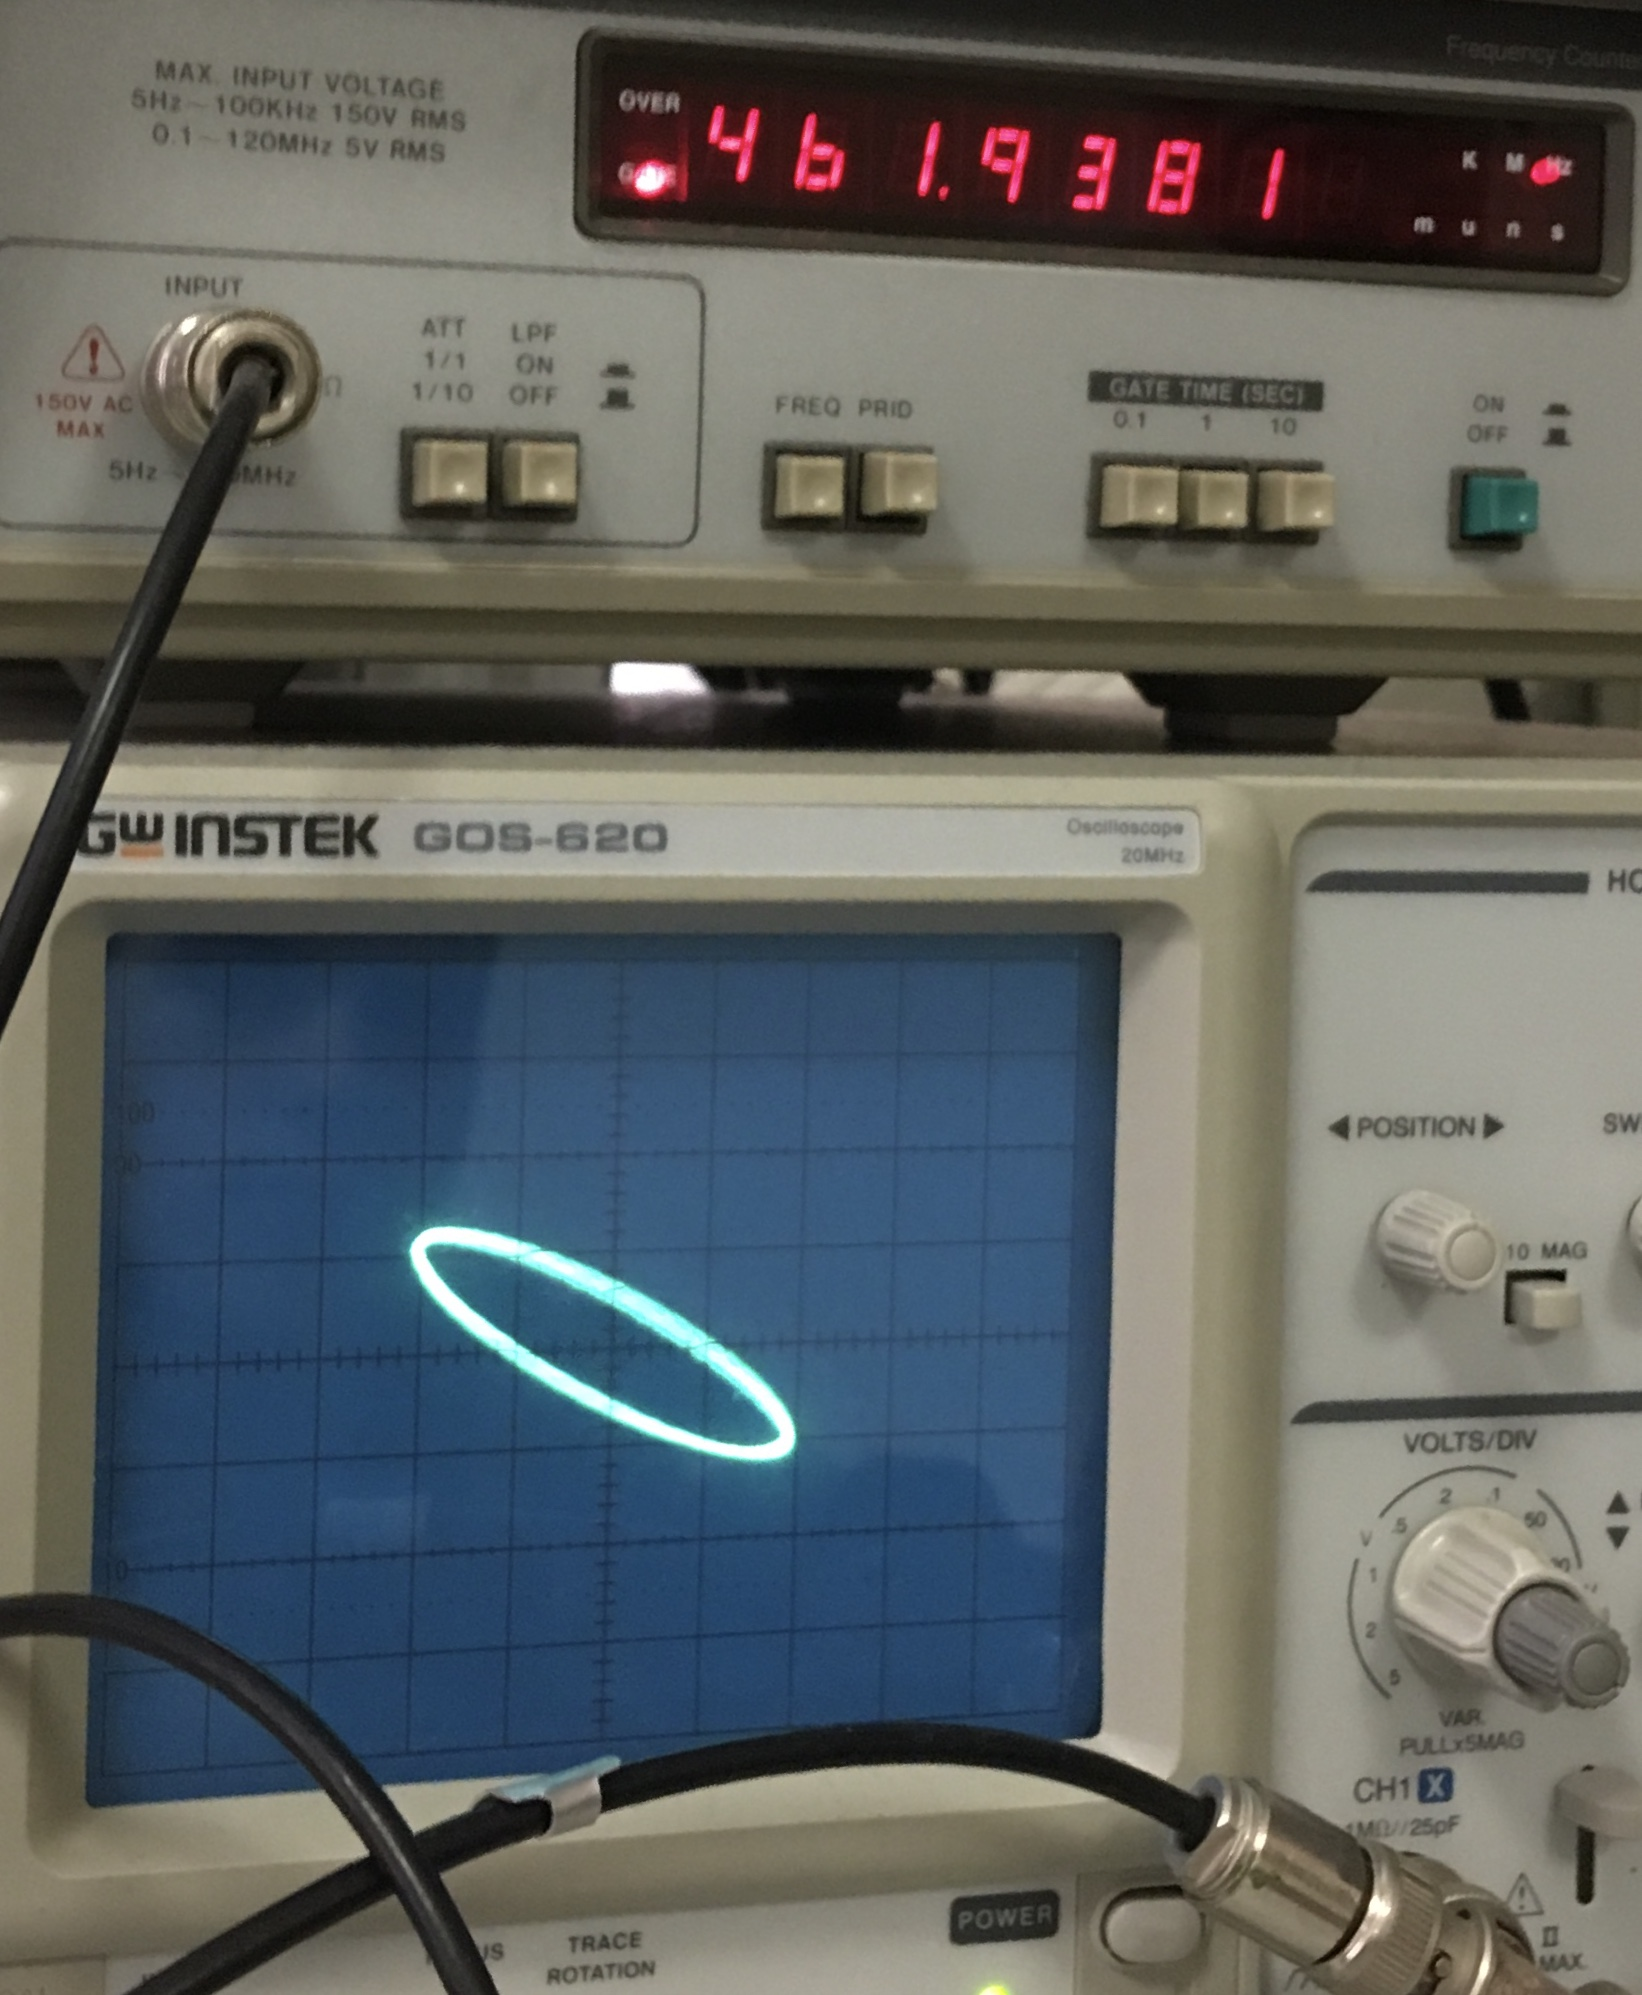
\includegraphics[width=0.8\linewidth]{IMG_5.jpg}\\

  Вращающийся ротор при подаче питания\\
 \end{center}
\end{minipage}
\begin{minipage}{0.4\textwidth}
\begin{center}
  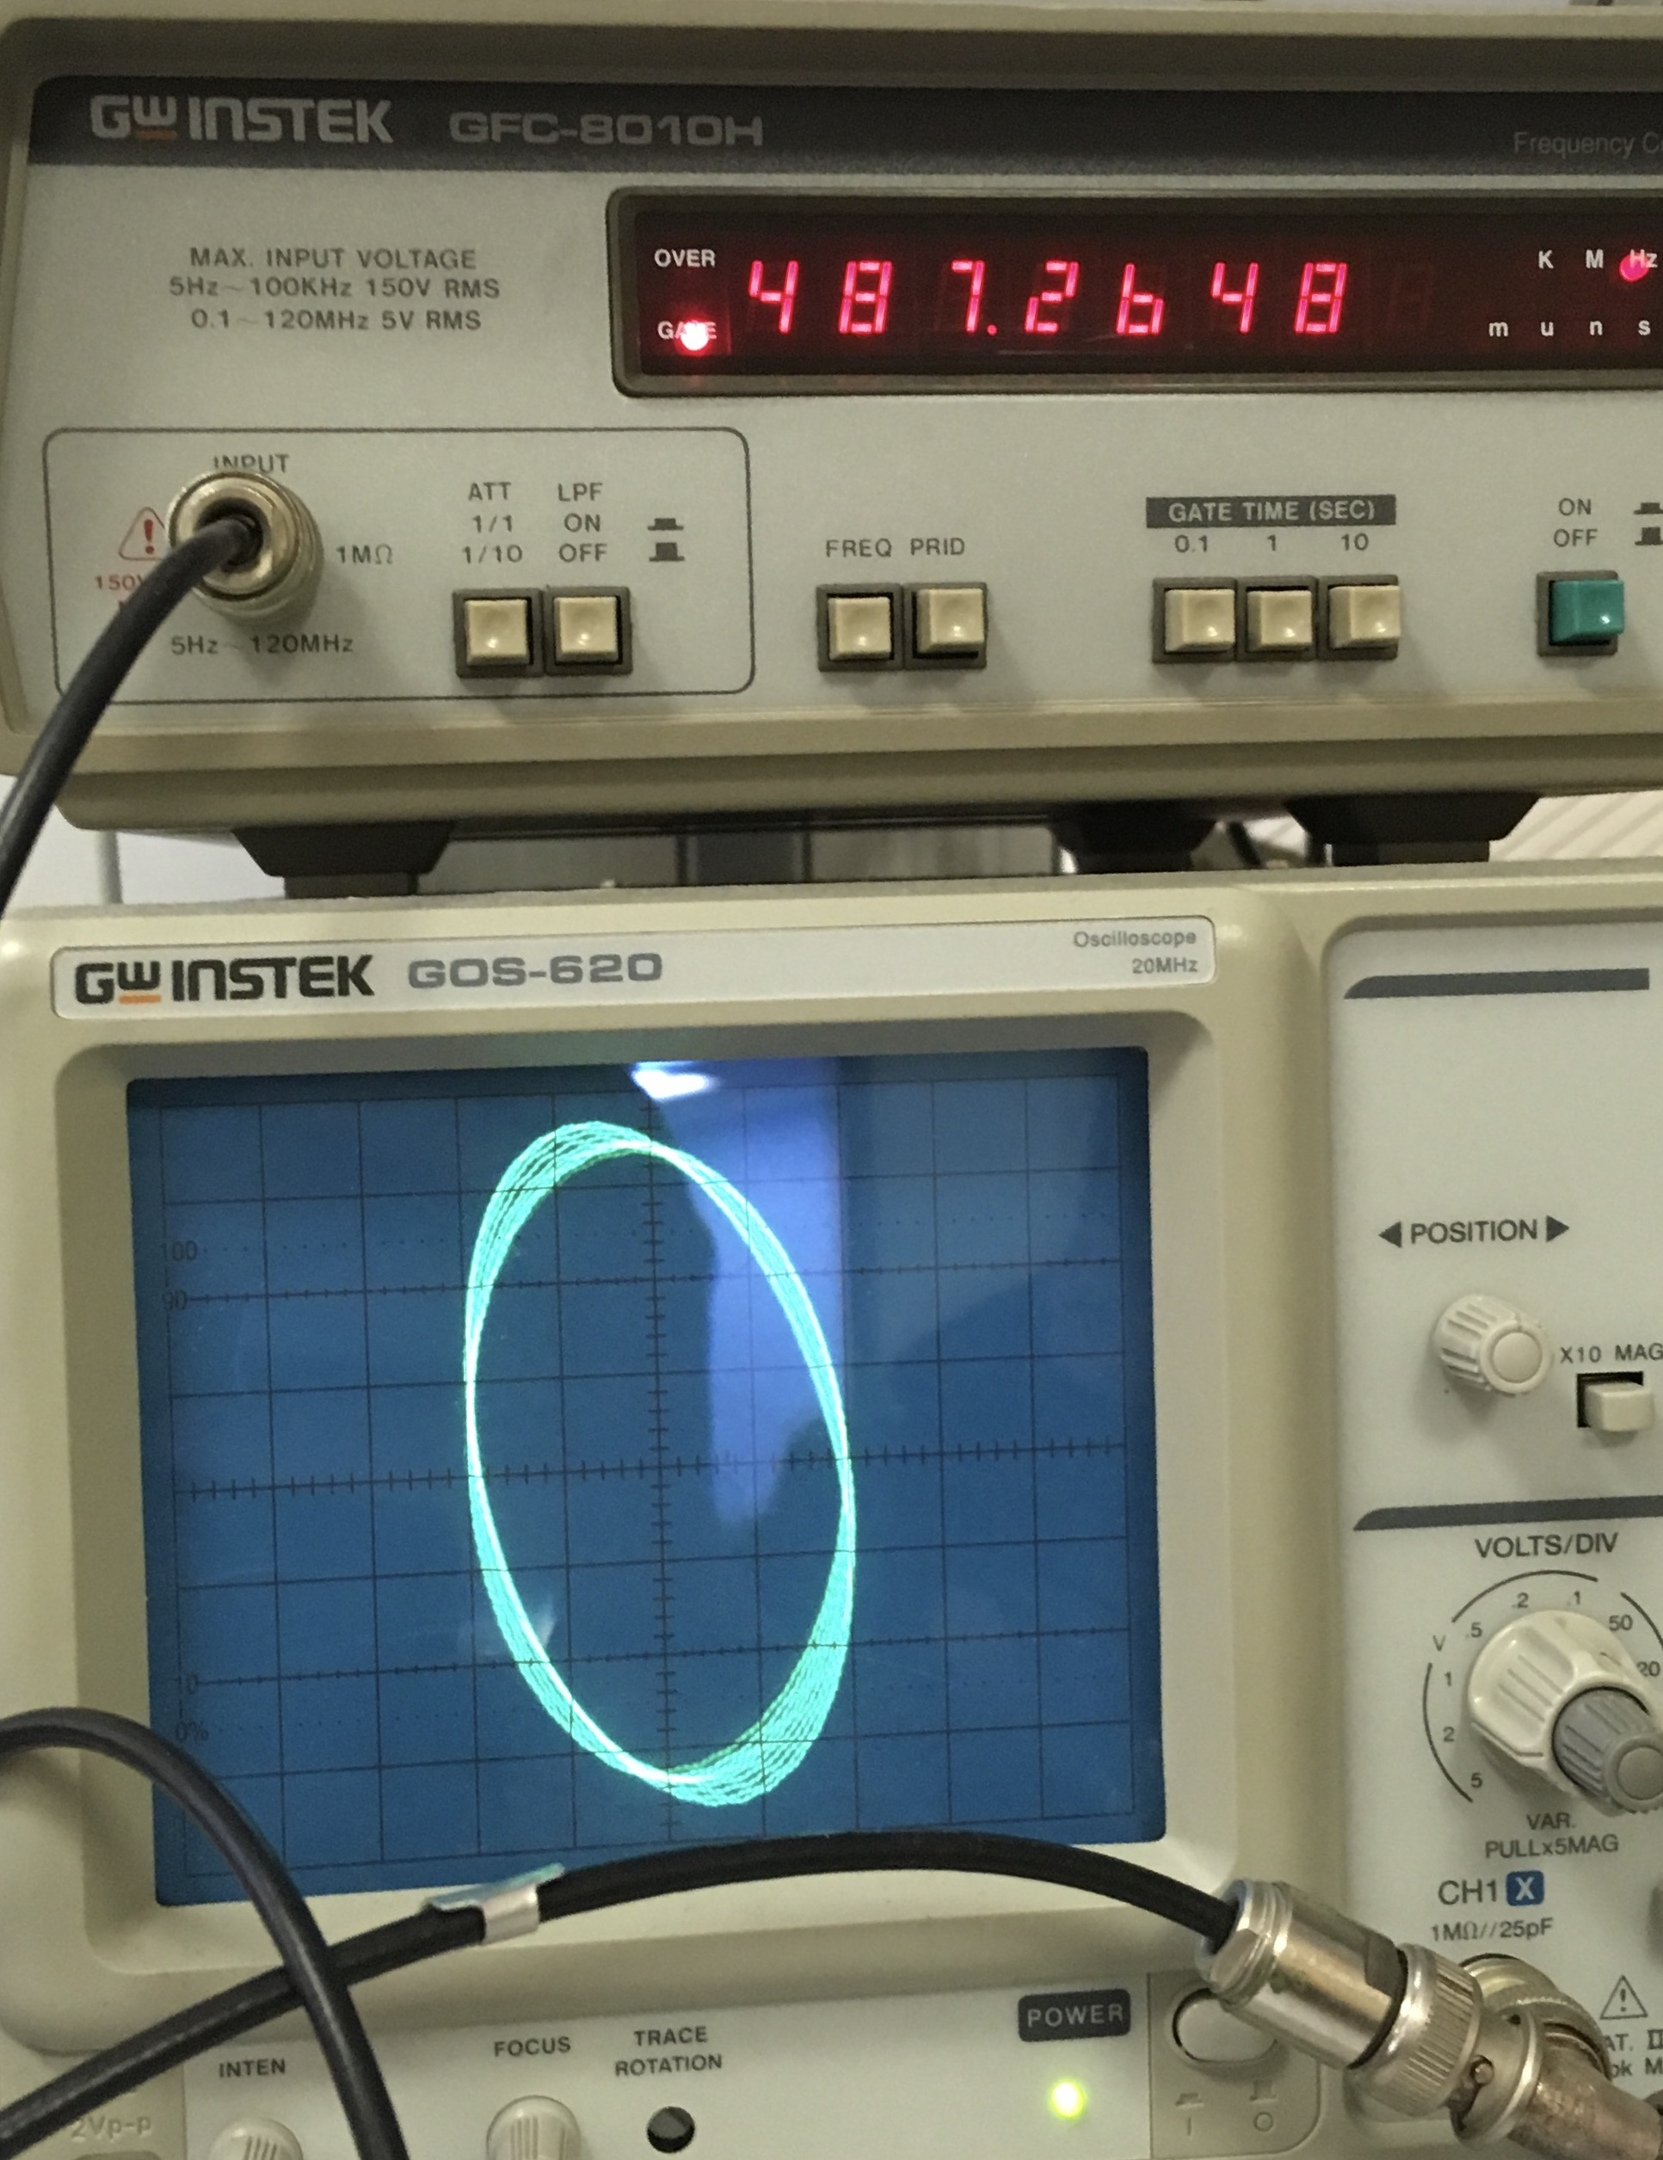
\includegraphics[width=0.8\linewidth]{IMG_6.jpg}\\
 
  Вращающийся ротор через небольшое время после выключения\\
 \end{center}
\end{minipage} 
  \end{center}

Из полученных на осциллографе результатов можно сделать вывод о том, что частота вращения ротора лежит в диапазоне $440 \pm 10$ Гц, к сожалению измерить частоту его вращения более точно не удалось. 

\section{Обсуждение результатов и выводы}
Измерение частоты вращения ротора гироскопа с помощью прецессии гироскопа совпало с измерением частоты вращения с помощью фигур Лиссажу. В первом способе погрешность измерения момента инерции рассчитывается по формуле:

\begin{align*}
\frac{\Delta I_2}{I_2} &= \sqrt{(\frac{\Delta I_1}{I_1})^2+4(\frac{\Delta T_1}{T_1})^2+4(\frac{\Delta T_2}{T_2})^2} = 3,2 \%\\
\frac{\Delta I_1}{I_1} &= \sqrt{(\frac{\Delta m}{m})^2+4(\frac{\Delta d}{d})^2} = 2,8\% \\
\end{align*}


Так как для каждого измерения вращения использовалась серия из 5 измерений, то необходимо учитывать случайную погрешность времени и угла.

\begin{align*}
\sigma_{сл_T} &= \frac{1}{N}\sqrt{\sum\limits_{i=1}^n(T-\bar{T})} \ (в \ пределах \ до \ 0,5  \ $\%$)\\
\sigma_{сл_\phi} &= \frac{1}{N}\sqrt{\sum\limits_{i=1}^n(\phi-\bar{\phi})} \ (в \ пределах \ от \ 0,3 \ до \ 1 \ $\%$) \\
\end{align*}

Полная погрешность считается по формуле\\

\begin{align*}
\sigma &= \sqrt{\sigma_{сл}^2 +\sigma_{сист}^2} \\
\end{align*}

Откуда получаем выражение для погрешности частоты вращения ротора гироскопа


\begin{align*}
\sigma_f &= \sqrt{\sigma_{сл}^2 + (\frac{\Delta I_2}{I_2})^2 +  (\frac{\Delta m}{m})^2 + (\frac{\Delta T}{T})^2} = 4\% \\
\end{align*}


\end{document}
